\documentclass[12pt,letterpaper]{exam}
\usepackage[lmargin=1in,rmargin=1in,tmargin=1in,bmargin=1in]{geometry}
\usepackage{../style/exams}

% -------------------
% Course & Exam Information
% -------------------
\newcommand{\course}{MAT 101: Exam 2}
\newcommand{\term}{Fall -- 2022}
\newcommand{\examdate}{11/21/2022}
\newcommand{\timelimit}{85 Minutes}

\setbool{hideans}{true} % Student: True; Instructor: False

% -------------------
% Content
% -------------------
\begin{document}

\examtitle
\instructions{Write your name on the appropriate line on the exam cover sheet. This exam contains \numpages\ pages (including this cover page) and \numquestions\ questions. Check that you have every page of the exam. Answer the questions in the spaces provided on the question sheets. Be sure to answer every part of each question and show all your work.} 
\scores
%\bottomline
\newpage

% ---------
% Questions
% ---------
\begin{questions}

% Question 1
\newpage
\question[10] As accurately as possible, plot the line $x= -\frac{5}{3}$ on the graph below.
	\[
	\fbox{
	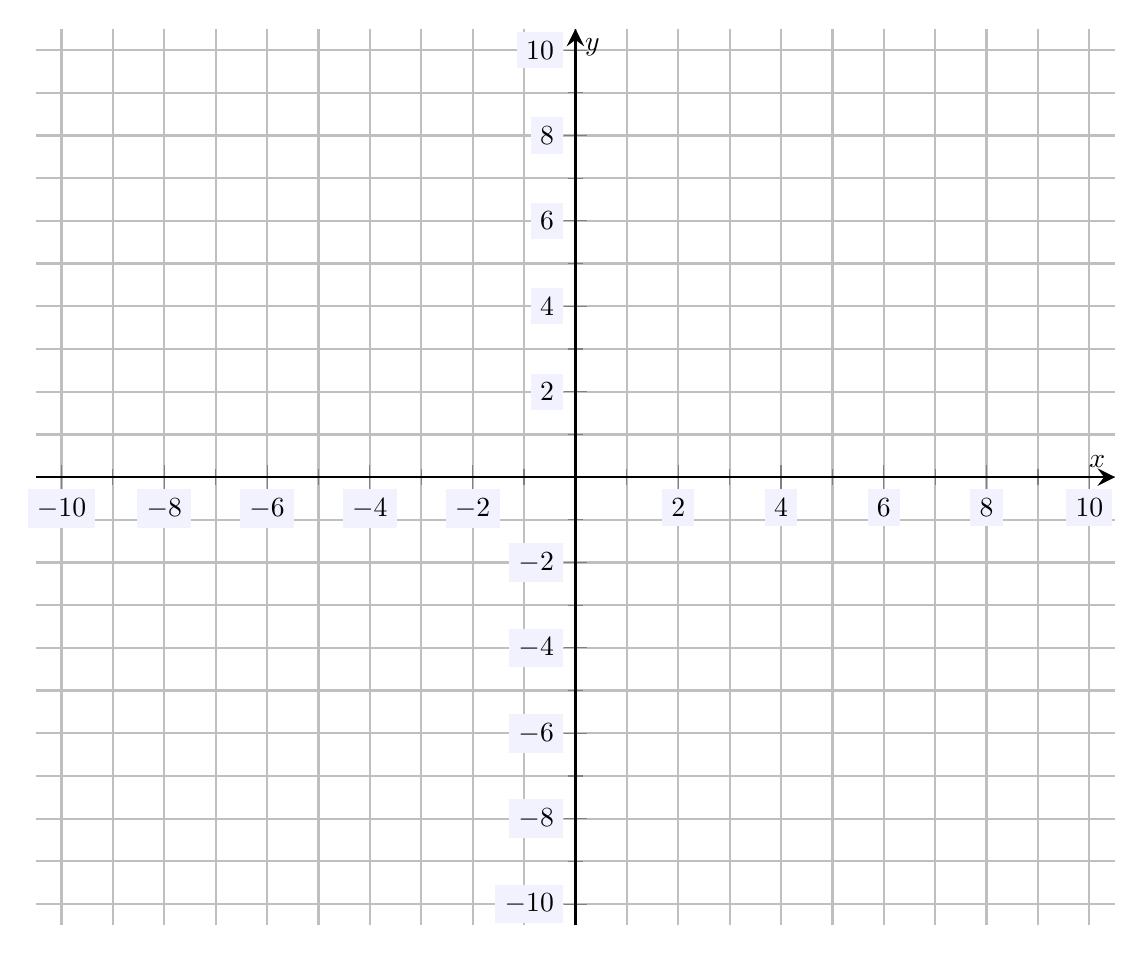
\begin{tikzpicture}[scale=2,every node/.style={scale=0.5}]
	\begin{axis}[
	grid=both,
	axis lines=middle,
	ticklabel style={fill=blue!5!white},
	xmin= -10.5, xmax=10.5,
	ymin= -10.5, ymax=10.5,
	xtick={-10,-8,-6,-4,-2,0,2,4,6,8,10},
	ytick={-10,-8,-6,-4,-2,0,2,4,6,8,10},
	minor tick = {-10,-9,...,10},
	xlabel=\(x\),ylabel=\(y\),
	]
	\end{axis}
	\end{tikzpicture}
	}
	\]



% Question 2
\newpage
\question[10] As accurately as possible, plot the line $y= \frac{3}{2}\, x - 3$ on the graph below. 
	\[
	\fbox{
	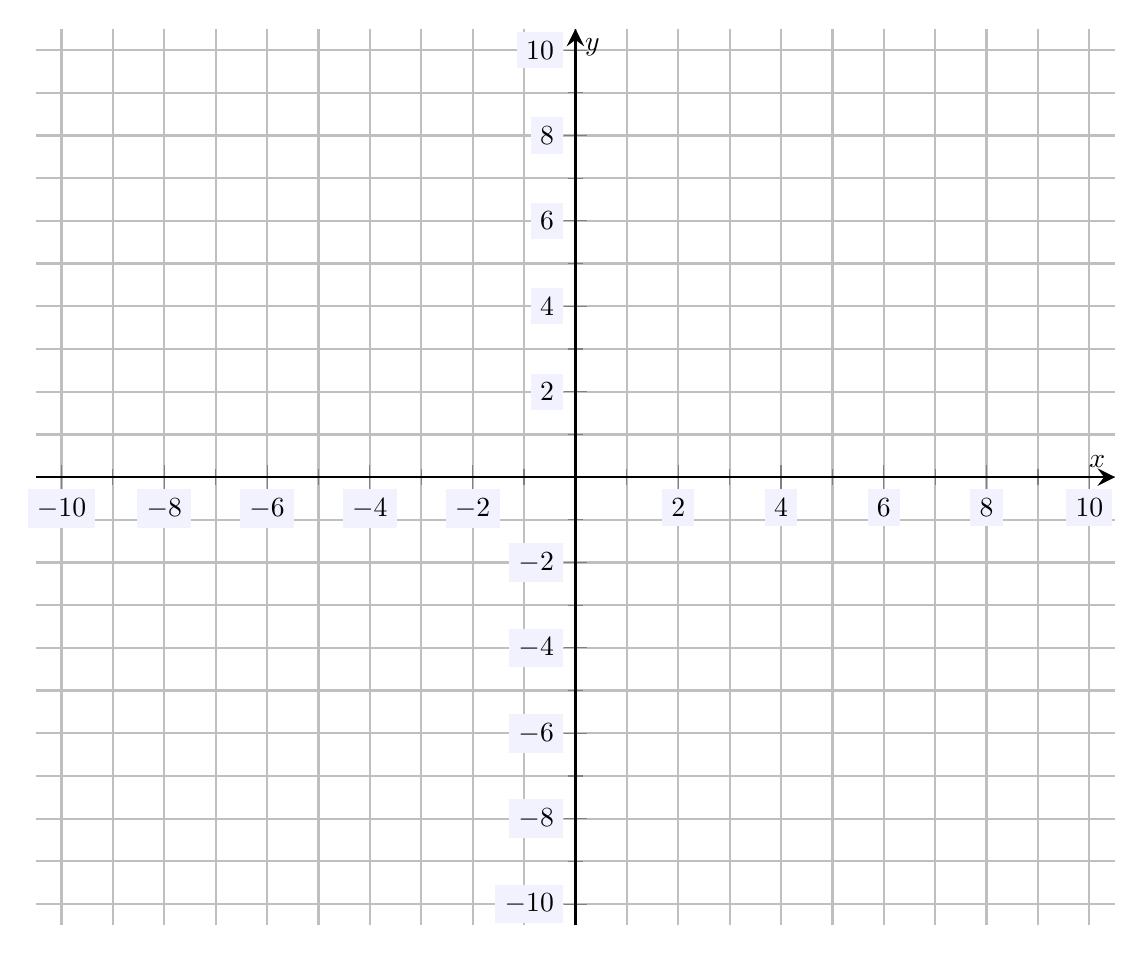
\begin{tikzpicture}[scale=2,every node/.style={scale=0.5}]
	\begin{axis}[
	grid=both,
	axis lines=middle,
	ticklabel style={fill=blue!5!white},
	xmin= -10.5, xmax=10.5,
	ymin= -10.5, ymax=10.5,
	xtick={-10,-8,-6,-4,-2,0,2,4,6,8,10},
	ytick={-10,-8,-6,-4,-2,0,2,4,6,8,10},
	minor tick = {-10,-9,...,10},
	xlabel=\(x\),ylabel=\(y\),
	]
	\end{axis}
	\end{tikzpicture}
	}
	\]



% Question 3
\newpage
\question[10] As accurately as possible, plot the line $5x + 4y= 10$ on the graph below. 
	\[
	\fbox{
	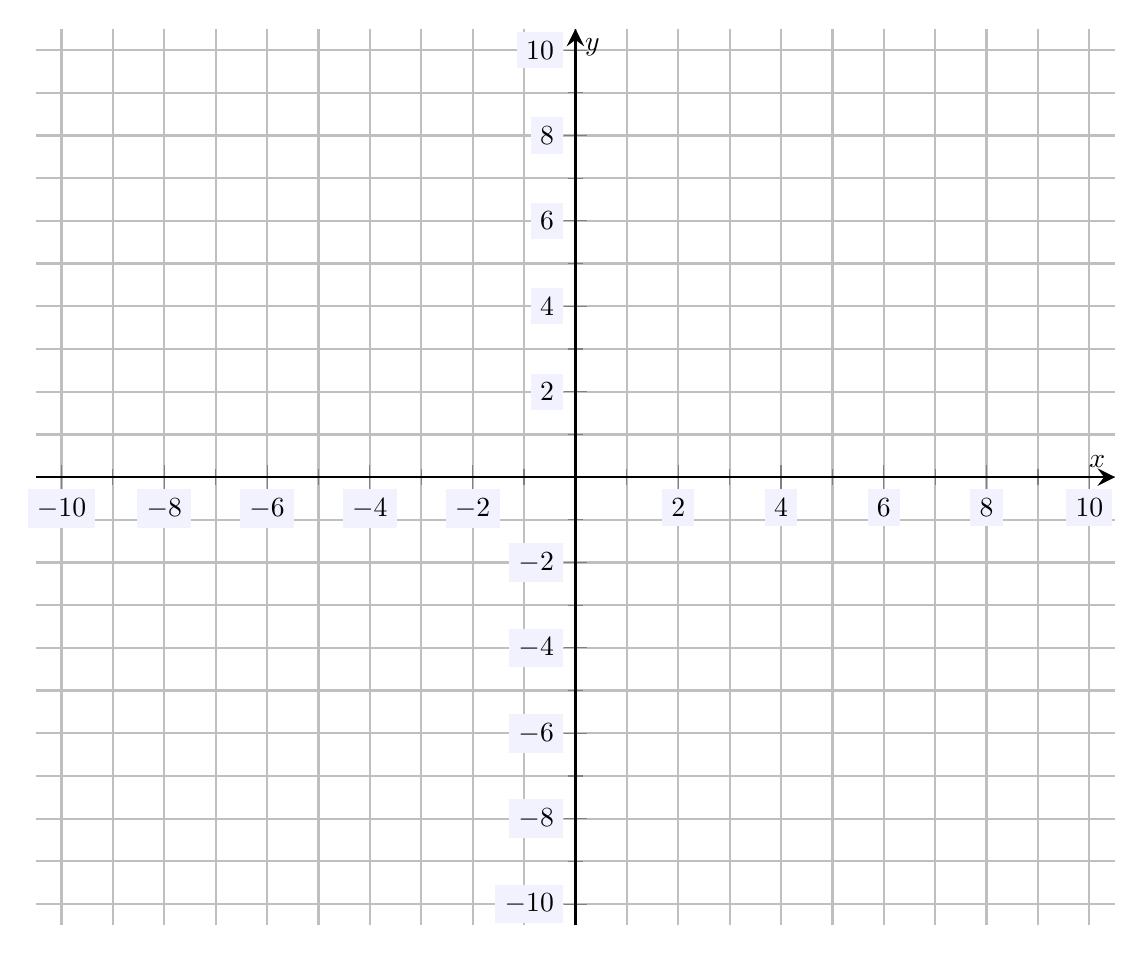
\begin{tikzpicture}[scale=2,every node/.style={scale=0.5}]
	\begin{axis}[
	grid=both,
	axis lines=middle,
	ticklabel style={fill=blue!5!white},
	xmin= -10.5, xmax=10.5,
	ymin= -10.5, ymax=10.5,
	xtick={-10,-8,-6,-4,-2,0,2,4,6,8,10},
	ytick={-10,-8,-6,-4,-2,0,2,4,6,8,10},
	minor tick = {-10,-9,...,10},
	xlabel=\(x\),ylabel=\(y\),
	]
	\end{axis}
	\end{tikzpicture}
	}
	\]



% Question 4
\newpage
\question[10] Consider the line given by $5x - 4y= 7$.
	\begin{enumerate}[(a)]
	\item Showing all your work and without referencing a graph, determine if $(-3, -2)$ is on the line. 
	\item Showing all your work and without referencing a graph, determine if $\big(1, -\frac{1}{2} \big)$ is on the line. 
	\end{enumerate}



% Question 5
\newpage
\question[10] Showing all your work and being sure to list the points, find at least three distinct points on the line $-7x + 3y= 10$. 



% Question 6
\newpage
\question[10] Consider the linear function $f(x)= 7 - \frac{6}{5}\,x$. Showing all your work, answer the following:
	\begin{enumerate}[(a)]
	\item Find the rate of change of $f(x)$.
	\item Interpret the rate of change of $f(x)$. 
	\item Determine whether $f(x)$ is an increasing or decreasing function.
	\item Determine the $y$-intercept of $f(x)$.
	\item Find the exact value of $f \big( \frac{2}{3} \big)$. 
	\end{enumerate}



% Question 7
\newpage
\question[10] Consider the linear function $f(x)= -3(2x - 7)$. Showing all your work, answer the following:
	\begin{enumerate}[(a)]
	\item Find the rate of change of $f(x)$.
	\item Interpret the rate of change of $f(x)$. 
	\item Determine whether $f(x)$ is an increasing or decreasing function.
	\item Determine the $x$-intercept of $f(x)$.
	\item Find an $x$-value such that $f(x)= 9$.
	\end{enumerate}



% Question 8
\newpage
\question[10] Find the equation of the line parallel to the line $y= 6 - x$ that has $x$-intercept $-12$. 



% Question 9
\newpage
\question[10] Find the equation of the line perpendicular to the line $y= -\frac{\pi}{2}$ that contains the $x$-intercept of the line $-7x + 5y= -3$.



% Question 10
\newpage
\question[10] Find the equation of the line that contains the $y$-intercept of $y= \frac{7}{11}\,x - 5$ and the point of intersection of $y= 4 - 3x$ and $y= \frac{1}{2}\,x + 18$. 



% Question 11
\newpage
\question[10] Showing all your work, find the solution to the following:
	\[
	2(x - 9)= \frac{x}{3} + 7
	\]



% Question 12
\newpage
\question[10] Showing all your work, find the solution to the following:
	\[
	\dfrac{5x - 3}{1 - x}= 13
	\]



% Question 13
\newpage
\question[10] Without explicitly finding the intersection, explain why the following lines $y= 2(7 - 5x)$ and $y= 5x + 2$ intersect. Showing all your work, find the intersection of the lines. 



% Question 14
\newpage
\question[10] Thai Tanic is a new restaurant chain that has been expanding across the Northwest. It is projected that next year, it will have \$800,000 in profits and the following year it will have \$1.2~million in profits. 
	\begin{enumerate}[(a)]
	\item Under what assumptions is a linear model to predict the growth rate of this business appropriate?
	\item Find a linear model for the profit of this company $t$ years from today. 
	\item Interpret the slope of your linear model in (b).
	\item Interpret the $y$-intercept of your linear model in (b), if possible. 
	\item How long until the company has a profit of \$5~million? 
	\end{enumerate}



% Question 15
\newpage
\question[10] Sia Gogh is driving down the highway at 65~mph. She has been driving for 2~hours. Sia determines her total distance traveled $t$~hours from now is approximately $D(t)= 65t + 130$. 
	\begin{enumerate}[(a)]
	\item Explain why her distance traveled is approximately linear.
	\item Interpret the slope of $D(t)$.
	\item Interpret the $y$-intercept of $D(t)$. 
	\item How far has she traveled after a total of 10~hours?
	\end{enumerate}


\end{questions}
\end{document}